\pretolerance=20000\tolerance=30000
\selectlanguage{spanish}
\pagestyle{fancy}
\chapter[Primer cap\'itulo]{Incluir el t\'itulo completo del primer cap\'itulo}\label{cap:1}
\vspace*{1cm}
\begin{center}
\begin{minipage}{12cm}
%------------------------------------------------
\texttt{\baselineskip 10pt
\begin{flushright}
pude introducir una cita\\
de su elecci\'on.\\
{\sf Autor de la cita.}
\end{flushright}}
%-------------------------------------
\textsl{\baselineskip 10pt
Escribir aqu\'i un resumen del primer cap\'itulo en el cual se describe el contenido, el objetivo y las principales referencias que se utilizaron.
Se incluye una adecuada justificaci\'on de porqu\'e es necesaria la presentaci\'on y desarrollo de este cap\'itulo.}
\end{minipage}
\end{center}

\section{Presentaci\'on de la tesis}%
Para una adecuada redacci\'on de la tesis es  \'util recordar algunos aspectos formales en la presentaci\'on final.\index{Presentaci\'on}
Por ejemplo, no s\'olo es preferible usar el lenguaje formal, sino tambi\'en tomar en cuenta que el estilo objetivo de los documentos acad\'emicos prioriza la redacci\'on en tercera persona: <<los autores consideran>> \, o <<se considera>>. \index{Presentaci\'on!estilo}
En este contexto, una vez terminada la redacci\'on formal es necesario realizar una revisi\'on final del trabajo, con una relectura cr\'itica  de todo el manuscrito para eliminar las posibles incoherencias en la redacci\'on, corregir y presentar el adecuado uso de los signos de puntuaci\'on y el acento, revisar el uso correcto de las reglas de la ortograf\'ia, presentar adecuadamente  los conectores y las preposiciones, etc.
En esta etapa, vale la pena revisar los aspectos formales tales como la forma adecuada de citar las referencias bibliograficas, entre otros.
%
\subsection{Ortograf\'ia}%
%
En la redacci\'on correcta de los p\'arrafos que componen la disertaci\'on final, se debe buscar la claridad y coherencia del texto, tomando en cuenta no solo al jurado, sino tambi\'en a cualquier  lector interesado de la tesis. \index{Ortograf\'ia}
Para lograr este objetivo es conveniente evitar la aparici\'on de errores ortogr\'aficos y el mal uso de los signos de puntuaci\'on.
Al respecto, la peque\~{n}a gu\'ia \cite{MR3052697} es de gran utilidad en la revisi\'on del estilo y la ortograf\'ia del texto matem\'atico; esta guia, entre otras cosas, incluye con claridad el uso adecuado de las letras may\'usculas.
De modo similar, en el libro \cite{da2016trabajo} se recomienda que las palabras clave en castellano deben incluirse con min\'uscula inicial (salvo que se trate de nombres propios o siglas).
Finalmente, se sugiere analizar y leer en detalle la \mbox{secci\'on 10} del tercer cap\'itulo  de \cite{da2016trabajo}, en la cual se presentan algunas recomendaciones pr\'acticas y apropiadas para evitar algunos errores ling\"{u}\'isticos frecuentes.
Por ejemplo, en la siguiente  oraci\'on  <<el teorema de Gauss--Bonnet, \emph{aparece} en el cap\'itulo 2>> se hace un uso incorrecto de la coma (la elección del idioma en la plantilla induce al uso adecuado de las comillas bajas, también conocidas como latinas, españolas o angulares).
%
\subsection{Orden de presentaci\'on}%
Las siguientes componentes son que se deberian incluir como parte de la tesis.
Algunas de ellas son opcionales y s\'olo se  consideran cuando sean necesarias.
%
\begin{verse}
(a) Caratula. \\
(b) Hoja de presentaci\'on y aprobaci\'on. \\
(c) Resumen ejecutivo (m\'aximo 500 palabras).\\
(d) Dedicatoria (opcional).\\
(e) \'Indice o Contenido.\\
(f) Lista de figuras (opcional).\\
(g) Agradecimientos (opcional).\\
(h) Introducci\'on.\\
(i) Cuerpo de la tesis.\\
(j) Conclusiones.\\
(k) Ap\'endices (opcional).\\
(l) Bibliograf\'ia\\
(m) \'Indice alfab\'etico (opcional).
\end{verse}
%
\subsection{Numeraci\'on y m\'argenes}%
En la descripci\'on anterior, los primeros \'items $a$, $b$, $c$, $d$, $f$ y $g$ tienen que ocupar \textbf{una p\'agina} (con excepci\'on del contenido) las que deben ser numeradas en romanos y con min\'usculas, $i$, $ii$, $iii$, $iv$, etc.
Espec\'ificamente, la numeraci\'on empieza en la introducci\'on y se hace con n\'umeros ar\'abigos, los cuales se colocan autom\'aticamente en la parte superior derecha.
Adem\'as, la introduci\'on  y las conclusiones deben estar igualmente citadas en (e), el contenido de la tesis.
\par
Respecto a los m\'argenes, la presentaci\'on final del trabajo de tesis debe hacerse en el formato $A4$ ($210\times297~mm$), a una sola cara en letra de tama\~{n}o $12$, en espacio simple con margen superior e inferior de $2.5$ $cm$ y margen en los lados de $3$ $cm$.
Cada uno de estos requerimientos formales, para la version digital del documento final de la disertaci\'on, se heredan directamente cuando se utiliza la presente plantilla y los comandos con los que ha sido dise\~{n}ada.
%
\subsection{Tablas y figuras}
Las tablas y figuras deben estar numeradas y citadas en el desarrollo del texto, adem\'as se incorporan dentro  del texto y no al final del cap\'itulo o en ap\'endices. Para ilustrar esta idea, a continuaci\'on se presenta la \mbox{figura \ref{gutu}} que incluye una tabla con algunos ejemplos del uso incorrecto de las may\'usculas dentro de la literatura matem\'atica.
Este ejemplo permite tambi\'en que se incluya, sin dificultad, la lista de figuras en las primeras p\'aginas de la tesis.
%
%%%%%%%%%%%%%%%%%%%%%%
\begin{figure}[htb]
\begin{center}
  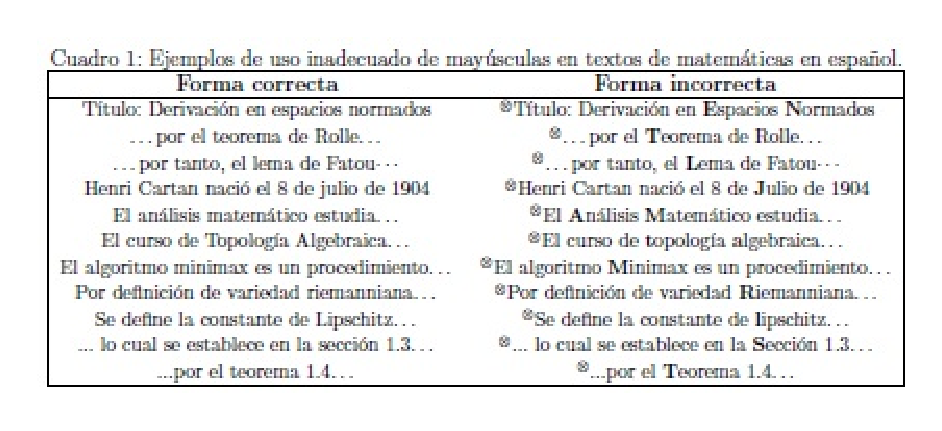
\includegraphics[width=14.5cm]{gutu.eps}
   \caption{Tabla tomada de \cite{MR3052697}}\label{gutu}
\end{center}
\end{figure}
%%%%%%%%%%%%%%%%%%%%%%%%%%%%%%%
%
\subsection{Cap\'itulos y ap\'endices}
Los cap\'itulos se enumeran con un n\'umero ar\'abigo y se recomienda incluir una mini-p\'agina con una descripci\'on del respectivo cap\'itulo.
Los ap\'endices se ordenan con letras may\'usculas $A, B, C \dots$ y debe aparecer en el contenido.
\par
Los niveles que se deben considerar son cap\'itulo, secci\'on, subsecci\'on y p\'arrafo; los cuales deben incluir lemas, proposiciones, teoremas y colorarios. Adem\'as, vale la pena ilustrar la exposici\'on  con \'utiles ejemplos.
Una herramienta que enriquece la redacci\'on consiste en enumerar los p\'arrafos no solo para citarlos y simplificar la exposici\'on, sino tambi\'en  para incluir solo aquellos que son necesarios en la redacci\'on clara y concisa del trabajo de tesis.
%
\begin{obs}
Para ilustrar el uso se escribe a modo de observación que las modificiones de la nueva carátula ya no incluyen el nombre de los jurados.
Sin embargo, estas deben aparecer en la hoja de presentación y para citar el nombre de cada uno se debe tener en cuenta la p\'agina \textsc{orcid} de cada integrante el jurado.
Consulte \texttt{https://orcid.org/} o bien \texttt{https://www.scopus.com/freelookup/form/author.uri}
\end{obs}
%
Las conclusiones aparecen al final con el comando \texttt{chapter*} y debe aparecer en el \'indice general.
\subsection{Bibliograf\'ia}%
La bibliograf\'ia se recomienda usar BibTEX en el estilo \texttt{amsalpha}, que produce etiquetas usando el nombre del autor y el a\~{n}o de la publicaci\'on.
El estilo \texttt{amsplain} genera números, pero en ambos casos se genera de modo automático sólo la bibliografia citada y con la información precisa para ubicarla en la literatura.
